\documentclass[ngerman,runningheads,a4paper]{llncs}
\usepackage{graphicx}
\usepackage{here}
\begin{document}

\title{Supporting Drum Learning/Playing through the use of Haptic Wearables}
\author{Simon Pfeifer}
\institute{Karlsruher Institut für Technologie, Institut für Telematik, Pervasive Computing Systems / TECO, Karlsruhe, Germany}
\maketitle

\begin{abstract}
Ein Musikinstrument zu Erlernen birgt einen großen Zeitaufwand, welcher vor dem Versuch abschrecken kann.
Haptische Wearables sollen den Lernprozess schneller und interessanter gestalten.
Das Schlagzeugspielen erfordert den Einsatz aller vier Gliedmaßen und ist deshalb zum testen von haptischen Wearables geeignet.
Dabei wird sich auf die Koordination, Zielsicherheit und Geschwindigkeit konzentriert.
Es besteht die Möglichkeit mit haptischen Wearables passiv zu lernen.
Grundlegende Entwurfsideen sind das Haptic Drum Kit, sowie die Haptic Bracelets.
Wobei die vibrotaktile Weste Einschränkungen aufzeigt.
Diese Arbeit soll einen Überblick über die aktuell existierenden Technologien und Entwicklungsmöglichkeiten geben und vergleicht die verschiedenen Ansätze.
\end{abstract}

\begin{keywords}
drum learning, haptic guidance, haptic wearables, passive learning
\end{keywords}

\section{Einleitung}
Das Erlernen eines Instruments ist ein langwieriger und traditionell mühsamer Prozess.
Nicht umsonst wird professionellen Musikern großer Respekt für ihr Talent gezollt.
Zudem fließt immenser Aufwand in das Erlernen eines instruments ein, der nicht zu vernachlässigen ist.
Seinem Idol nachzueifern ist daraufhin der logische Schritt.
Nach dem Kauf eines Instruments folgen die ersten Versuche, die nicht ansatzweise and das herankommen, was sich vorgestellt wurde.
Entweder der Versuch wird wieder aufgegeben, oder es wird sich Hilfe geholt.
Die Hilfe besteht vielleicht aus einem Lernvideo.
Doch dieses ist viel zu schnell und auch nach vielen Versuchen kommt man nicht an das gezeigte Ergebnis heran.
Der nächste Schritt ist dann ein professioneller Lehrer, der individuell auf den Schüler eingeht, Fehler direkt erkennt und korrigiert.
So wird das Lernen effektiv und die Erfolge, durch das abschließen kleiner Lernschritte, motivieren zum Weitermachen.
Doch der Weg zu einem guten Musiker ist lang und aufwendig.
Daher die Frage, ob das nicht auch schneller und damit effizienter geht.
Neue Lernmethoden werden immer wieder ausprobiert und zeigen nicht selten Erfolge.
Ein gutes Beispiel dafür sind alternative Schulsysteme.
Die Idee besteht darin auch neue Lernmethoden für das Erlernen eines Instruments zu finden.
Mittlerweile sind haptische Wearables kompakt, technisch ausgereift und bezahlbar.
Somit bieten sich der Versuche an, das Lernen eines Instruments mit diesen Wearables zu unterstützen oder komplett zu übernehmen.
Diese Arbeit beschäftigt sich mit diesem Gedanken und beschränkt sich dabei auf das Schlagzeug als Perkussionsinstrument, bei dem der ganze Körper verwendet wird und eine große Fläche für Wearables bietet.
Dafür werden erst Grundlagen geklärt und anschließend Studien analysiert, um herauszufinden, ob haptische Wearables in der Lage sind das Erlernen des Schlagzeugspielens zu erleichtern.
Können haptische Wearables einen professionellen Lehrer ersetzen?
Kann passiv während der Ausführung anderer Aktivitäten gelernt werden?
Wie verhält sich das haptische Lernen im Vergleich zu auditiven oder visuellen Lernen?
Diese Fragen werden in Angriff genommen und bilden das Grundgerüst dieser Arbeit.



\section{Grundlagen}
\subsection{Haptik}
Haptik ist im Duden als die "Lehre vom Tastsinn"\cite{Haptik} definiert und kommt vom griechischen h\'{a}ptein, das für heften, berühren und angreifen steht. Das adjektiv haptisch bedeutet "den Tastsinn, das Tasten betreffend, auf dem Tastsinn beruhend, mithilfe des Tastsinns [erfolgend]"\cite{haptisch}. Haptik steht also für die Wahrnehmung und Manipulation durch Berührung.

Haptische Wahrnehmung lässt sich in taktile und kinetische Informationenen unterteilen. Taktile Informationen beinhalten das Gefühl des Kontakts durch die Rezeptoren auf der Haut, die unter und um den Kontaktpunkt liegen. Kinetische Informationen sind die Positionen und Bewegungen der Körperteile die durch die Berührung und die damit verbundenen Kräfte entestehen. \cite{srinivasan1995haptics}

Haptisches Feedback lässt sich in haptisches, tactiles und force-feedback unterteilen.
Haptisch ist dabei nur das Feedback, welches signalisiert, dass ein Kontakt besteht. Taktiles Feedback gibt Auskunft über den ausgeübten Druck oder eine Bewegung.
Force-feedback ist eine Kraft, die die eigene Bewegung beeinflusst, wenn keine Gegenkraft ausgeübt wird.
Ein Joystick mit force-feedback entwickelt entsprechend der eingehenden Informationen eine Kraft in eine Richtung, die dann auf den Benutzer übertragen wird und dieser nachgibt, oder eine Gegenkraft aufbringen muss.
So kann durch force-feedback ein Widerstand simuliert werden, der die Immersion steigert.\cite{bennett2004hap}



\subsection{Wearables}
"Wearables sind kleine, am Körper getragene Computer, die, verbaut in die Kleidung oder Accessoires, mitlaufen, ohne aktiv bedient werden zu müssen." \cite{kleine2016gesellschaftliche}
Für Wearables gibt es zahlreiche Definitionsversuche, sodass keine allgemeingültige Definition existiert. In diesen Versuchen lassen sich allerdings ähnliche Merkmale ausmachen. So sind Wearables während des Tragens immer einsatzbereit, können also jederzeit benutzt und wieder ignoriert werden, ohne dass sie abgeschaltet werden müssen. Wearables laufen im Hintergrund und müssen nicht im Mittelpunkt stehen. Der Nutzer kann sich auf sein Gerät konzentrieren, wenn er es benötigt und es läuft sonst im Hintergrund mit. Nebenbei nehmen Wearables druch Sensoren Informationen aus der Umwelt auf und können diese verarbeiten und weiterkommunizieren.\cite{kleine2016gesellschaftliche}

Die wichtigsten Funktionen von Wearables sind Tracking, Monitoring, Communication und Augmentation. Das Tracking beschränkt sich dabei nicht nur auf GPS Koordinaten, sondern auch die Aufnahme von Bewgeungsabläufen, wie Augenbewegungen bei Eye-Trackern oder Armbewegungen um Schritte zu zählen. Beim Monitoring geht es um Vitalfunktionen wie Blutdruck, oder Puls und Verhaltensmuster wie zum Beispiel das Schlafverhalten. Die Kommunikation von Wearables ist nicht nur auf Kommunikation mit dem Nutzer beschränkt sondern schließt auch die Kommunikation mit anderen Wearables, Computern und Programmen ein. So sollen sich Wearables mit anderen Geräten verbinden können, um bestimmte Funktionalitäten zu erfüllen. Zudem entsteht so auch die Möglichkeit von Mensch zu Mensch Interaktionen über Wearables durch Anrufe, Kurznachrichten oder E-Mails. Die letzte große Funktion ist die Augmentation, wobei Wearables durch eingebaute Sensoren die Umwelt aufnehmen und so eine Augmented Reality erschaffen können, um dem Nutzer zur Umwelt passende Zusatzinformationen zur Verfügung zu stellen.\cite{kleine2016gesellschaftliche}

Die Anforderungen an Wearables sind sehr hoch, da sie im Hintergrund ohne besonderen Fokus durch den Nutzer funktionieren sollen. Daher muss der Tragekomfort hoch sein, um langes und unterbewusstes Nutzen zu ermöglichen.
Das Nutzungsgebiet von Wearables ist sehr weitläufig wodurch ein hoher Anspruch an die Funktionalität geht. Ein Nutzer möchte nicht für jede Tätigkeit ein anderes Wearable tragen müssen, sondern alle Funktionen in einem Gerät haben.
Zusätzlich ist das Design entscheidend für eine intuitive und fortwährende Nutzung.\cite{kleine2016gesellschaftliche}

Die am weitesten verbreiteten Wearables sind Head-Mounted Display, wie Datenbrillen zum Beispiel Google Glasses oder Hololens, Armbänder und Smart Watches wie Fitnessarmbänder, die Körperfunktionen wärend dem Sport messen oder Smart Watches, die verbunden mit einem Smartphone viele Funktionen des Geräts am Handgelenk bieten. Dazu kommt noch Intelligente Kleidung, die durch eingebaute elektronische Geräte Vitalparameter misst, den Standort überwacht oder den Träger wärmt.\cite{kleine2016gesellschaftliche}

Wearables sind in Eingabe und Ausgabe nur auf die eingebauten Sensoren und verbundene Geräte beschränkt. So können Eingaben über Sprachbefehle durch das Mikrofon, Zeichen über Touchscreen oder Tastatur, Gesten durch Beschleunigungssensoren oder Bilder durch eine Kamera erfolgen. Genauso kann auch die Ausgabe über alle möglichen Kanäle erfolgen. Visuell über einen Bildschirm, auditiv durch Lautsprecher oder verbundene Kopfhörer und haptisch durch Vibration.
\cite{kleine2016gesellschaftliche}

\subsection{Haptische Wearables}
Ein Wearable mit programmierbaren haptischen Sensoren wird haptisches Wearable genannt.
Die am meisten verwendeten haptischen Wearables sind mit vibrotaktilen Sensoren ausgestattet, wie man sie von Videospielfernbedienungen und Smartphones kennt. Dies sind einfache Vibratoren, deren Frequenz und Amplitude sich anpassen lässt.
Wodurch verschiedene Signale kodiert werden können. So kann eine kurze, aber starke Vibration gegen eine lange, aber schwache Vibration unterschieden werden und so verschiedene Nachrichten übermittelt werden.
Eine weiterentwickelte Variante ist das force-feedback. Hierbei wird eine Kraft aufgebracht, die eine Gegenkraft erfordert, oder das berührende Körperteil bewegt. Ein Beispiel hierfür sind Joysticks oder Lenkräder, die sich entsprechend der aktuellen Situation bewegen und so echte Kräfte simulieren.\cite{bennett2004hap}

\subsection{Schlagzeugspielen}
Ein Schlagzeug besteht aus einer Kombination von Schlaginstrumenten. Das Standardschlagzeug besteht aus einer großen Trommel, einer kleinen Trommel, mehreren Toms, einer Hi-Hat und verschiedenen Becken. Zum spielen eines Schlagzeugs werden im Normalfall Trommelstöcke aus Holz verwendet. Für die Basstrommel gibt es eine Fußmaschine. Als Alternative zu Trommelstöcken werden auch Besen verwendet, die aus gebündelten Stöckchen bestehen.

Das Lernen des Schlagzeugspielens ist besonders schwer, da ein Schlagzeug kein einzelnes Instrument ist, sondern ein System aus Instrumenten, die mit Händen und Füßen erreichbar sein müssen. Der wesentliche Bestandteil des Lernprozesses ist die Hand-Fuß-Koordination.\cite{bouwer2011haptic}
Das Schlagzeugspielen lässt sich als schnelle, koordinierte Bewegung aller Gliedmaßen nach bestimmten Mustern beschreiben.
Dabei muss jeder Schlag mit hoher Treffgenauigkeit und der richtigen Stärke zum richtigen Zeitpunkt erfolgen.\cite{6775447}

Der Lernvorgang geschieht normalerweise praktisch an einem Musikstück. Es werden Taktart und Form des Stückes herausgehört, analysiert und erlernt.
Durch professionellen Unterricht kann der Lernprozess unterstützt werden.
Dabei werden Schlagzeugnoten beigebracht sowie wichtige Grundkentnisse der allgemeinen Musiklehre und die richtige Körperhaltung.
Der Hauptteil von Unterrichtsstunden besteht aber aus dem korrekten und flüssigen lernen von Rhythmen.\cite{6775447}

\section{Studien zum Lernen mit Haptischen Wearables}


\subsection{Haptic Guidance System}
Wie in \cite{4479984} nachzulesen, vergleicht Graham Grindlay in seiner Arbeit von 2008, wie gut sich ein einfacher Rhythmus mit haptischer Führung im Vergleich zu auditiven Lernen, erlernen lässt.
Dabei beschreibt er die Ähnlichkeit seiner Konstruktion zu dem Führen der Hand des Schülers durch den Lehrer.
Zu dieser Methode greifen viele Lehrer, weil das verbale Beschreiben nicht ausreicht, um eine komplizierte Bewegung genau zu erklären.
Allerdings entspricht das Führen nicht unbedingt der exakt richtigen Bewegung und ist eingeschränkt, was Geschwindigkeit und Stärke angeht.
Graham Grindlay will mit seinem Haptic Guidance System die Bewegungsgenauigkeit und -geschwindigkeit verbessern und das Lernen erleichtern.

\subsubsection{Aufbau}
Wie man in Fig. \ref{hagus} sehen kann, besteht das Haptic Guidance System aus einem Rotationsmotor, an dem ein Trommelstock befestigt ist.
Der Benutzer legt seinen Arm in die dafür vorgesehene Schiene, wo er fixiert wird, um die richtige Handgelenksposition sicherzustellen.
Unter der Spitze des Trommelstocks befindet sich eine Trommel, die bei der Benutzung bespielt wird.
Der Rotationsmotor kann von der Konstruktion getrennt werden, um ohne Widerstand spielen zu können.
Ebenso kann mit und ohne Rotationsmotor die Bewegung auf einem Computer aufgenommen und wieder abgespielt werden.
Zudem ist das System mit Sicherheitsmaßnahmen ausgestattet.
Zum einen sind Einschränkungsstangen installiert, um eine unnatürliche Bewegung des Handgelenks zu verhindern und zusätzlich gibt es noch einen Knopf um das System sofort zu stoppen.

\subsubsection{Teilnehmer}
Für das Experiment haben sich 32 Rechtshänder gemeldet. 20 davon Frauen und 12 Männer. Kein Teilnehmer hatte Erfahrung im Spielen von Perkussionsinstrumenten.

\subsubsection{Ablauf}
In diesem Experiment wurden vier verschiedene rhythmische Aufgaben verwendet. Jede dieser Aufgaben war nicht trivial, aber lernbar in den Versuchsperioden.
Die Rhythmen wurden mit dem Haptic Guidance System für den Computer und auf Audio aufgenommen, damit sich der Rhythmus der Teilnehmer genauso, wie das Beispiel anhören kann.
Jeder Teilnehmer sollte einen Rhythmus nur mit Audio lernen, einen nur mit Haptischer Führung ohne Audio, einen mit Haptischer Führung und Audio und den letzten mit Haptischer Führung, Audio und Kopfhörer mit Störgeräuschen.
Jede Lernphase für einen Rhythmus bestand aus zweimaligen Vorführen und direkt danach dem Nachspielen durch den Teilnehmer.


\subsubsection{Ergebnisse}
Die Aufnahmen der Teilnehmer wurden in zeitlicher Präzision und Aufschlaggeschwindigkeit verglichen.
Im Bezug auf zeitliche Präzision zeigt die Kombination von Audio und Haptik einen Vorteil gegenüber Audio oder Haptischer Führung, durch eine geringere Fehlerrate von 10\%.
Zudem führte haptische Führung alleine zu mehr Fehlern beim Timing.
Bei Aufschlaggeschwindigkeit zeigt sich ein klarer Nachteil des Audio Trainings, da die Aufnahmen, die mit haptischer Führung geübt wurden, im Durchschnitt 11\%  weniger Fehler beinhalten.
Die Kombination von Audio und haptischer Führung erreichte sogar 17\% weniger Fehler als das Audio Training.
Allerdings weisen die Daten zum Lernen mit haptischer Führung eine größere Varianz auf, als das kombinierte Training mit Audio und haptischer Führung.
Die Arbeit kommt zu dem Schluss, dass die Kombination von Audio und haptischer Führung zum besten Erfolg führt und sich eine Langzeitstudie zu dem Thema anbietet.

\begin{figure}[H]
  \centering
  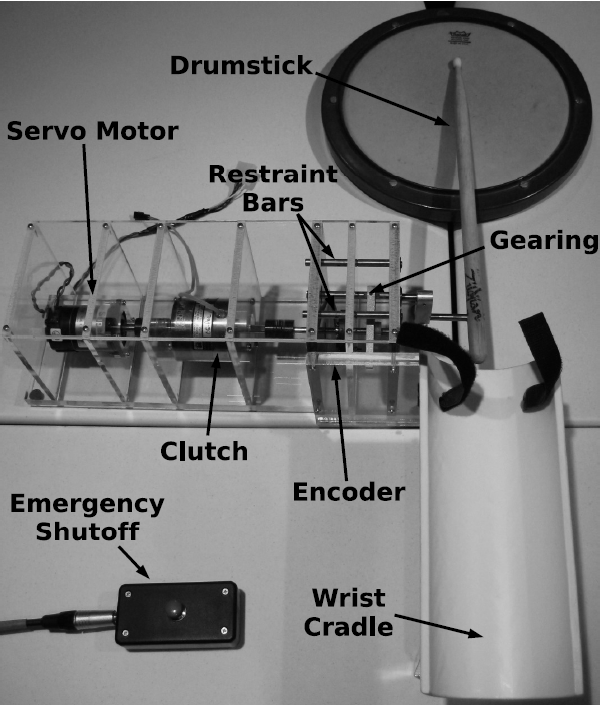
\includegraphics[width = 0.5\textwidth]{pictures/hapticdrumstick1}
  \caption{The Haptic Guidance System \cite{4479984}}
  \label{hagus}
\end{figure}

\subsection{Haptic Drum Kit}
In diesem Abschnitt geht es um das Haptic Drum Kit von Simon Holland, Anders J. Bouwer, Mathew Dalgleish und Topi M. Hurtig \cite{10.1145/1709886.1709892}
.
Die Arbeit über das Haptic Drum Kit beschäftigt sich mit der Frage, ob sich polyphone Rhythmen, für die man mehrere Gliedmaßen koordinieren muss, durch Vibratoren an den Handgelenken und Knöcheln erlernen lassen.
Unter polyphonen Rhythmen versteht man Rhythmen, die sich aus mehreren einfachen Rhythmen zusammensetzen, welche unterschiedlich schnell sein können und so einen komplexeren neuen Rhythmus ergeben.
Die Wissenschaftler untersuchen die Frage, ob Anfänger komplexe Rhythmen nur mit haptischen Reizen lernen können.
Zudem werden die Ergebnisse des haptischen Lernens mit den Erfolgen nach auditiven Lernen und Lernen mit gleichzeitigen auditiven und haptischen Reizen gemessen.

\subsubsection{Aufbau}
In Fig. \ref{hapkit2} zu sehen, besteht das Haptic Drum Kit aus 4 Vibratoren, die mit elastischen Bändern an den Handgelenken und Knöcheln befestigt werden.
Die Sensoren werden an den Gliedmaßen angebracht, weil keine Transferleistung mehr nötig sein soll, um den richtigen Arm, oder das richtige Bein zu bewegen.
Die Kabel von Armen und Beinen werden an einer Bauchtasche zusammengeführt und von dort mit einem Computer verbunden, wie in Fig. \ref{hapkit1} zu sehen.
Mit dem Computer werden die Vibrationsgeräte angesteuert und der Benutzer soll nach diesen haptischen Signalen spielen.
Als Schlagzeug wird ein Midi drum kit verwendet, um die zeitliche Genauigkeit des Benutzers am Computer messen zu können.

\subsubsection{Teilnehmer}
Für die Studie wurden fünf männliche Teilnehmer getestet. 4 waren Anfänger und einer hatte fünf Jahre Erfahrung vom Spielen in einer Band und Unterrichtsstunden.

\subsubsection{Ablauf}
Zu Beginn stellte jeder Teilnehmer das Schlagzeug ein, sodass alle Trommeln getroffen werden konnten.
Danach wurden 20 Rhythmen aus vorbereiteten Rhythmen zufällig ausgewählt und dem Teilnehmer vorgespielt, der versuchen sollte, diese nachzuspielen.
Die Teilnehmer wurden dabei aus drei Winkeln gefilmt und beobachtet.
Nach der Testphase wurd eine Befragung durchgeführt, um die Meinungen der Teilnehmer zu erfahren.
\subsubsection{Ergebnisse}
Die Befragung der Teilnehmer zeigte, dass alle gewillt waren, das System wieder zu benutzen.
Zudem gaben alle an, dass es einfacher war den Audioaufnahmen zu folgen und auch im Tempo zu bleiben.
Wobei durch die haptische Führung schneller klar war, welches Körperteil zu bewegen ist.
Die Teilnehmer bevorzugten die Kombination von auditiven und haptischen Lernen.
Da es sich um eine Designstudie handelt, wurden viele Verbesserungvorschläge eingebracht.
Die Vibratoren waren zu laut und die Vibration teilweise zu schwach und wurde so von der Bewegung des Schlages übertönt, was in der Arbeit "haptic masking" genannt wird.
Genauso können bei schnellen Rhythmen mehrere Vibrationen zu einer verschwimmen, was auch zum "haptic masking" zählt.
Die Geräte sollten sich individuell einstellen lassen.
Durch die Gleiche Vibrationsintensität war auch schwer festzustellen, wo der Rhythmus beginnt, oder zur Wiederholung ansetzt.
Eine interessante Beobachtung war, dass beim haptischen Lernen manche Teilnehmer parallel gelernt haben, statt jede Bewegung alleine.
Eine neue Version des Haptic Drum Kits mit verbesserten Vibratoren, die stärker und zeitlich präziser funktionieren und sich individuell einstellen lassen, könnte schon viele Probleme der ersten Version beheben.

\begin{figure}[H]
  \centering
  \begin{minipage}[b]{0.4\textwidth}
    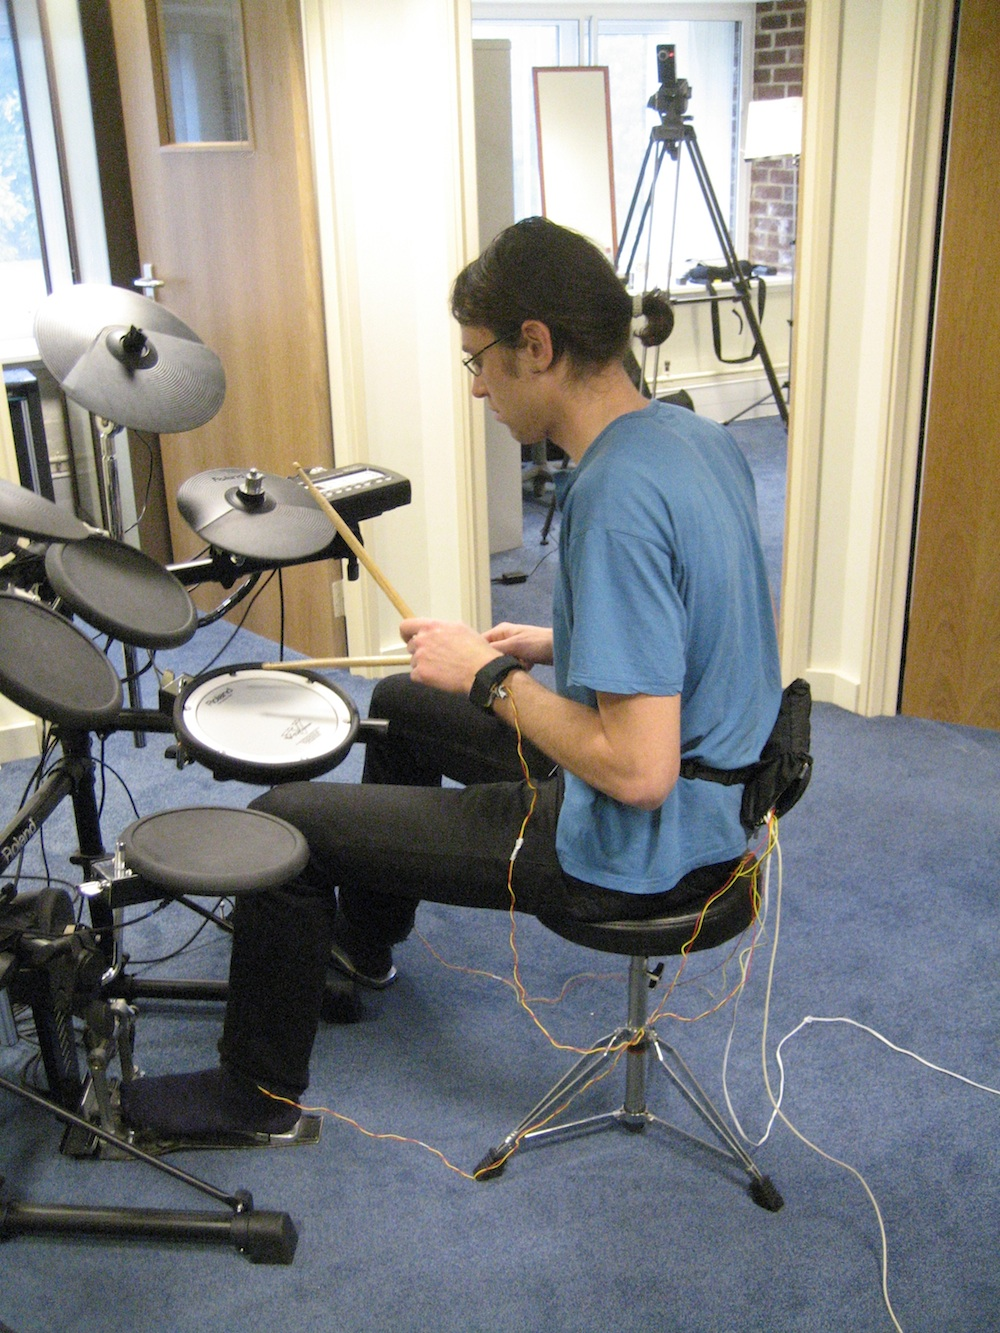
\includegraphics[width = \textwidth]{pictures/hapticdrumkit}
    \caption{Haptic Drum Kit \cite{10.1145/1709886.1709892}}
    \label{hapkit1}
  \end{minipage}
  \hspace{0.1\textwidth}
  \begin{minipage}[b]{0.4\textwidth}
    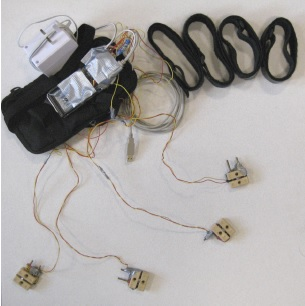
\includegraphics[width = \textwidth]{pictures/hapticdrumkit1}
    \caption{Vibratoren mit Bändchen und Tasche \cite{10.1145/1709886.1709892}}
    \label{hapkit2}
  \end{minipage}
\end{figure}


\subsection{Haptic iPod / Haptic Bracelets}
Die Arbeiten von Bouwer, Dalgleish und Holland \cite{bouwer2011haptic}, \cite{bouwer2013haptic} basieren auf den Ergebnissen zum Haptic Drum Kit \cite{10.1145/1709886.1709892} und beschäftigen sich mit der Frage, ob sich mehrgliedrige Rhythmen auch passiv lernen lassen. In diesem Abschnitt wird auf diese Arbeiten eingegangen.
Dabei werden lautlos rhythmische Reize über die Vibratoren abgespielt, während sich die Teilnehmer mit einer anderen Aufgabe beschäftigen.
Das verwendete System wird Haptic iPod genannt. In einer späteren Veröffentlichung wurde der Name in Haptic Bracelets geändert, wegen der möglichen Fehlleitung durch Produkte der Firma Apple.
\subsubsection{Aufbau}
Der Haptic iPod existiert in zwei verschiedenen Versionen.
Eine portable Feldversion mit im Vorhinein aufgenommenen vierspurigen Stücken und batteriebetriebenen Kopfhörerverstärkern.
Dazu noch eine statische Testversion die mit einem Laptop bedient wird und mit stärkeren Kopfhörerverstärkern ausgestattet ist.
Für die Studie wurde die statische Testversion verwendet, weil sie stärkere Signale ermöglicht und am Computer steuerbar ist.

\subsubsection{Ablauf}
Die Teilnehmer spielten zu Anfang möglichst schwere Rhythmen nach Gehör.
Danach wurden 2 Rhythmen aus den gespielten Rhythmen ausgewählt und abwechselnd über die haptischen Wearables abgespielt, während eine 30 minütige Leseverständnis Aufgabe bearbeitet wurde.
Im Anschluss sollten die Rhythmen vom Anfang wiederholt werden.
Die Ergebnisse wurden auf Genauigkeit, Timing, Anzahl der Versuche und Fehleranzahl im besten Versuch verglichen.
Zum Schluss wurden die Probanden zu ihren Erfahrungen und Einstellungen zum Haptic iPod befragt.

\subsubsection{Ergebnisse}
Das Experiment zeigte drei besondere Ergebnisse.
Haptische Führung kann mit ähnlichem Erfolg, wie Audioführung verwendet werden.
Die Kombination von beiden Methoden ist gegenüber einer einzelnen zu bevorzugen.
Wie beim Haptic Drum Kit \cite{10.1145/1709886.1709892} ist die Haptik gegenüber dem Gehör im Vorteil, wenn es darum geht, welche Gliedmaßen zu verwenden ist.
Die haptische Führung hat keinen Vorteil, wenn es darum geht, welche Trommel zu spielen ist.
Die Teilnehmer gaben an, dass die Wearables über die Zeit unangenehm zu tragen waren.
Verbesserungvorschläge waren hier die Kombination von auditiven und haptischen Lernen währen der passiven Lernphase. Sowie Portabilität und Kabellosigkeit.
Das passive Lernen macht es auch schwerer sich auf eine Aufgabe zu konzentrieren und fordert das setzen von Prioritäten.

\subsection{Vibrotaktile Weste}
In Lee und Seungmoon Choi \cite{6775447} verwenden eine Weste und Bänder an den Knöcheln, die mit vibrotaktilen Geräten ausgestattet sind, um neun mögliche Schlaginstrumente eines Schlagzeugs abzubilden. Die natürlich egozentrische Anordnung der Geräte ermöglicht eine intuitive Verbindung eines Reizes mit dem Treffen eines bestimmten Schlaginstruments. Das System verfügt über die Möglichkeit, zwei verschiedene Schlagstärken zu signalisiren, durch Veränderung der Intensität und Dauer der Vibration. In der Studie kommt das Schlagzeug nicht zum Einsatz, da in einem Vorversuch festgestellt wurde, dass motorische Fehler der unerfahrenen Teilnehmer die Messergebnisse verfälschen würden.

\subsubsection{Aufbau}
In Fig. \ref{vest} sieht man den Aufbau der Studie. Dieser besteht aus einem Computer mit 24 Zoll Bildschirm zur visuellen Repräsentation der vibrotaktilen Reize, einem Midi-Drum Kit, der vibrotaktilen Weste, sowie den Knöchelbändern.
Die selbstkonstruierte Weste und Knöchelbänder bestehen aus elastischen Gummibändern, an die mithilfe von Metallklemmen, ERM Motoren geheftet sind. Sieben Taktoren befinden sich an der Weste und jeweils ein Taktor and den Knöchelbändern.
Durch die Verwendung von Klemmen, lassen sich die Taktoren individuell für jeden Teilnehmer an der Weste befestigen, da es hilfreich ist eine stabile Verbindung zwischen Taktor und Körper herzustellen.
Die Taktoren sind and den Knöcheln nach vorne angebracht, um die Bewegung zur Bedienung des Pedals nicht einzuschränken.

\subsubsection{Teilnehmer}
Für die Studie haben sich 12 männliche Teilnehmer zwischen 19 und 28 Jahren mit einem Altersschnitt von 21 Jahren gemeldet. Alle Teilnehmer haben keine körperlichen Einschränkungen und besitzen keine Vorkenntnisse im Schlagzeugspielen.

\subsubsection{Ablauf}
Zuerst musste der Teilnehmer lernen die Reize richtig zu erkennen, da die Erkennungszeit die maximale Spielgeschwindigkeit begrenzt.
Dafür sollte der Teilnehmer nach dem fühlen eines haptischen Reizes den zu der Stelle passenden Punkt auf dem Bildschirm anklicken.
Das Bild entspricht dem ersten Bild in Fig. \ref{vest2}. Bei einem schwachen Signal sollte der Punkt mit der linken Maustaste angeklickt werden und bei einem starken Signal mit der rechten Maustaste. So konnte sich der Teilnehmer an das System gewöhnen, auftretene Probleme behoben werden und die Verarbeitungsperformance verlässlicher gemessen werden.
Danach begann die dreiteilige Testreihe mit Messungen.
Der erste Test sollte die Zeit zwischen Spüren und Aktion messen. Auf dem Bildschirm wurde dem Teilnehmer die Position und Stärke des nächsten Reizes angezeigt um die Identifikationszeit zu minimieren. Zufällig wurde der Reiz in den folgenden eins bis drei Sekunden abgespielt und der Teilnehmer sollte so schnell, wie möglich klicken.
Der zweite Test schloss die Identifikation mit ein. Der Teilnehmer sah auf dem Bildschirm das zweite Bild aus Fig. \ref{vest2}. Nach dem Spüren eines Reizes sollte er die richtige Position mit der richtigen Maustaste anklicken, wie im Testdurchlauf vor den Messungen. Durch das gespiegelte Bild eines Körpers sollte die Entscheidungszeit minimiert werden.
Im letzten Test wurde auch die Entscheidungszeit gemessen, also die gesamte Dauer vom Spüren eines Reizes bis zur Aktion. Als Hintergrund wurde ein Schlagzeug dargestellt, wie im dritten Bild von Fig. \ref{vest2} zu sehen ist.
In allen Testszenarien befanden sich die zu klickenden Punkte an den gleichen Positionen auf dem Bildschirm. Jeder Test bestand aus 180 Reizen, um alle Positioen und Stärken mit 10 Wiederholungen zu messen. Zudem haben die Teilnehmer währen der Test Ohrstöpsel getragen, um nicht durch Geräusche aus der Umwelt abgelenkt zu werden.


\subsubsection{Ergebnisse}
In die Messungen sind nicht nur die Zeiten eingeflossen, sondern auch die Korrektheit der Antworten. Die Teilnehmer trafen zu 95\% die richtigen Antworten und benötigten 0,91 Sekunden für die Verarbeitung eines Reizes. Davon werden 0,3 Sekunden für die Erkennung, 0,46 Sekunden für die Identifikation und 0,15 für die Aktion benötigt. Dichtes Platzieren der Taktoren erhöhte signifikant die benötigte Identifikationszeit und längere neuronale Übertragungsdistanz führte zu längeren Erkennungszeiten.



\begin{figure}[H]
  \centering
  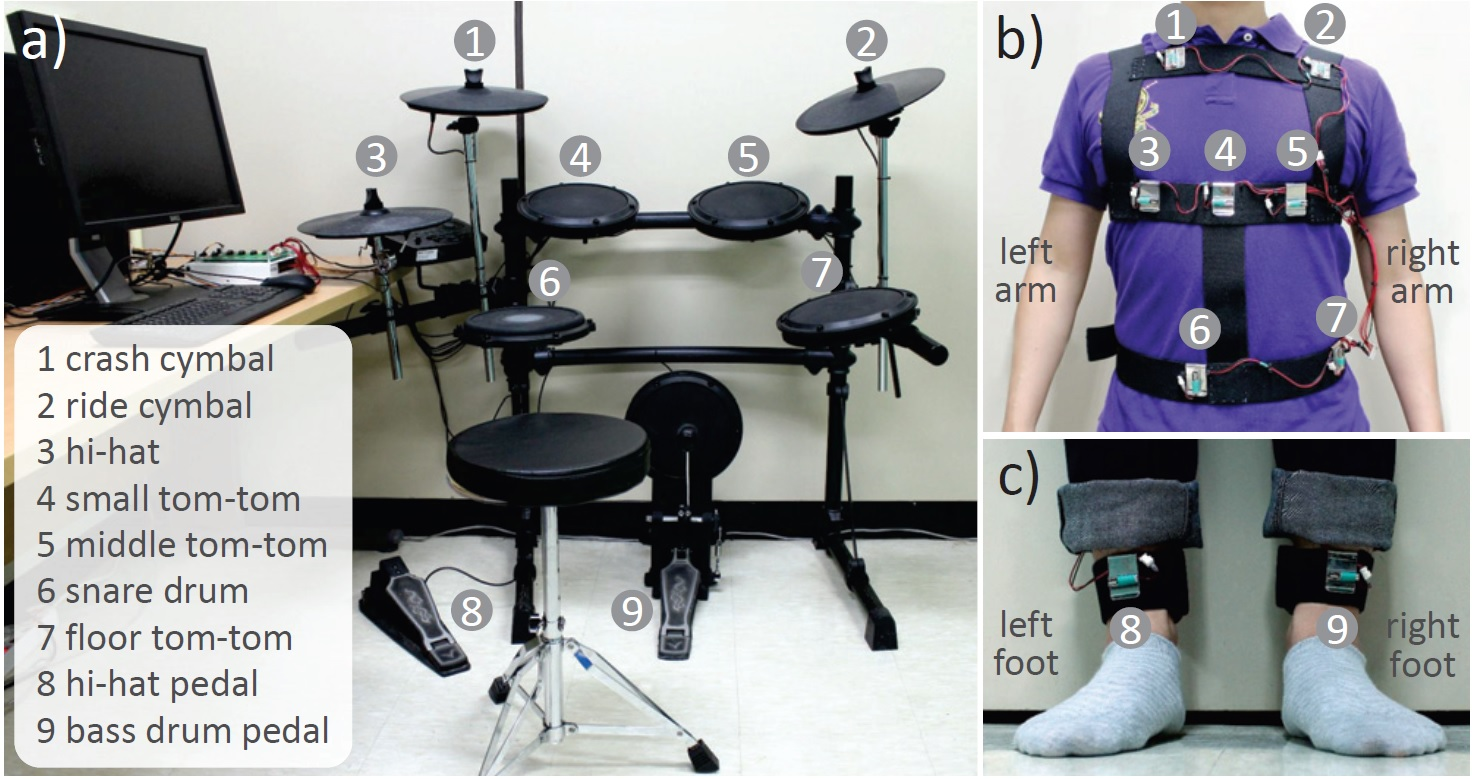
\includegraphics[width = \textwidth]{pictures/vibrotactilevest2}
  \caption{Vibrotaktile Weste mit Knöchelbändern und Midi-Drum Kit\cite{6775447}}
  \label{vest}
\end{figure}

\begin{figure}[H]
  \centering
  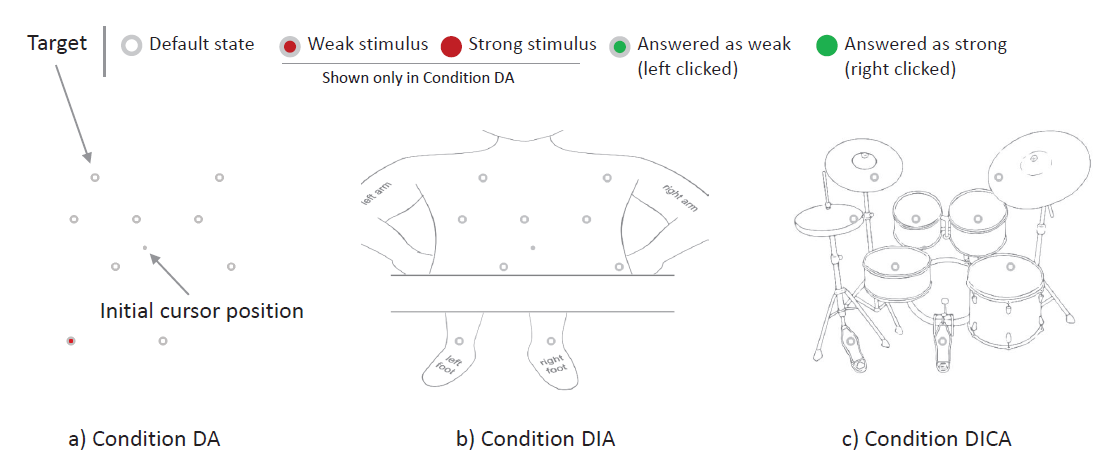
\includegraphics[width = \textwidth]{pictures/vestpc}
  \caption{Visuelle Szenen für den Bildschirm\cite{6775447}}
  \label{vest2}
\end{figure}


\section{Zusammenfassung}
\subsection{Fazit}
Diese Arbeit zeigt verschiedene Ansätze haptische Wearables zu verwenden, um das Schlagzeugspielen zu lernen. Für einen komplexen Prozess wie diesen, ist aber noch keine perfekte Lösung entstanden. Für einzelne Teile des Schlagzeugspielens sind erfolgsversprechende Experimente durchgeführt worden. So zeigt das Haptic Drum Kit \cite{10.1145/1709886.1709892}, dass haptische Wearables dabei helfen können, die richtigen Gliedmaßen zu verwenden und polyphone Rhythmen mit dieser Unterstützung lernen lassen. Allerdings werden visuelle oder auditive Hilfen benötigt, um den Rhythmus richtig zu verstehen und die richtige Trommel, oder das richtige Becken zu treffen.

 Die logische Folge ist die verschiedenen Konstruktionen miteinander zu kombinieren, um alle Aspekte des Schlagzeugspielens abzudecken. Allerdings lassen sich, durch die schnelle Abfolge von vibrotaktilen Reizen, diese nicht mehr eindeutig voneinander trennen und das gleichzeitige Identifizieren von mehreren Reizen erfordert eine starke mentale Leistung und somit auch mehr Zeit. Der Effekt des "haptic masking" \cite{10.1145/1709886.1709892} und die Ergebnisse zur vibrotaktilen Weste zeigen, dass eine Kombination nicht möglich ist. Dadurch ist die Geschwindigkeit des Stückes stark eingeschränkt und das System nicht nur anstrengend zu bedienen sondern auch nur bei Anfängern anwendbar. Haptische Wearables als Lernunterstützung sind für Teile des Lernprozesses anwendbar, bringen aber keine Zeitersparnis gegenüber herkömmlichen Lernmethoden.

Haptisches Lernen kann das herkömmliche Lernen nach Gehör und Lehrer bis jetzt nicht ersetzen, bietet aber eine interessante zusätzliche Lernmöglichkeit, um Abwechslung in das Lernen zu bringen.
Das passive Lernen nur mit haptischen Wearables ist auch nicht möglich, da nicht alle benötigten Informationen bereitgestellt werden können.

\subsection{Ausblick}
Mit neuen Entdeckung in der Forschung zu Wearables, die kompakter und effizienter sind, lassen sich in Zukunft neue Versuche starten, das Schlagzeugspielen nur mit haptischen Wearables zu lernen. Ein Beispiel hierfür ist VibroTac, ein Armband mit mehreren vibrotaktilen Aktoren, die sich individuell steuern lassen und vom Benutzer erkannt und unterschieden werden können. Das Armband wurde getestet als Assistenzgerät für Blinde und visuell eingeschränkte Personen, um Kollisionen zu vermeiden.
In der Zukunft können Haptische Wearables in Gesundheit, Unterhaltung, Sicherheit und vielen weiteren Gebieten, die noch nicht identifiziert und untersucht wurden, eingesetzt werden.
Derzeitige Vibrationsgeräte in Smartphones könnten durch verschiedene Rhythmen mehr Informationenen übertragen.
Außerdem können haptische Wearables Verwendung in weiteren physisch komplexen Fähigkeiten wie Tanzen, Sport oder Medizin finden. %( remote medicine)


\bibliographystyle{splncs03}
\bibliography{proseminar}
\end{document}
